\titre{Question 1}\\
\\
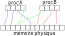
\includegraphics{Images/fig19.pdf}
\\
\newpage
\titre{Question 2}\\
\\
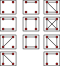
\includegraphics[width=200px]{Images/fig20.pdf}
\\
\\
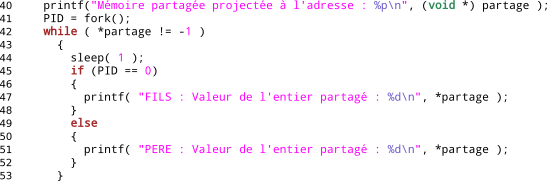
\includegraphics[width=300px]{Images/fig21.pdf}
\\
\titre{Question 3}
\begin{enumerate}
	\item $K_n$ possède $\frac{n(n-1)}{2}$ arêtes.
	\item $\bar{K_n}$ possède 0 arête
	\item $O(n^2)$
\end{enumerate}

\titre{Question 4} Il y a deux sous graphes isomorphes à $K_3$ et aucun isomorphe à $\bar{K_3}$
\newpage
\titre{Question 5} \\
\\
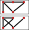
\includegraphics[width=100px]{Images/fig23.pdf}
\\
\titre{Question 6} 
\begin{enumerate}
	\item .\\ 
\includegraphics{Images/fig24.pdf}
	\item $O(n^2)$
	\item .\\
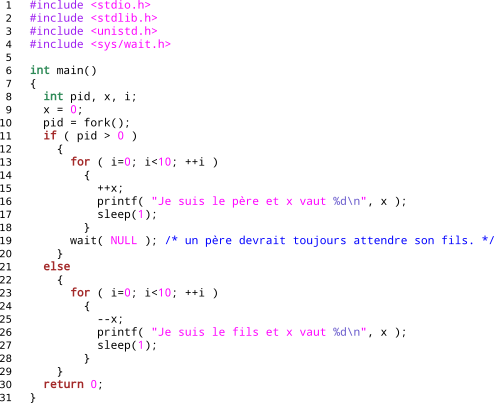
\includegraphics{Images/fig25.pdf}
	\item $O(n^2)$
	\item Faire mieux ???
\end{enumerate}

\titre{Question 7} Il faut commencer par enlever une allumette \\
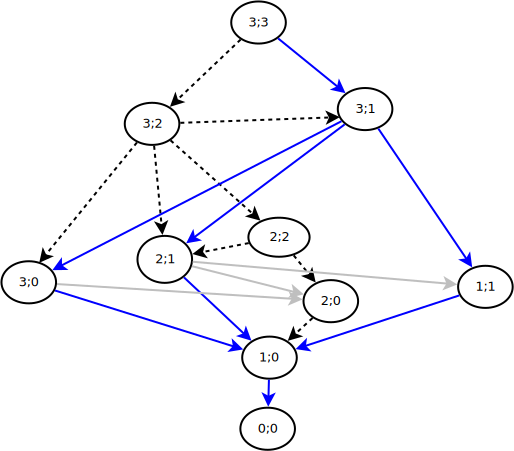
\includegraphics[width=250px]{Images/fig26.pdf} \\

\titre{Question 8} P = passeur, C = choux, B = chèvre (bêêê), L = loup \\
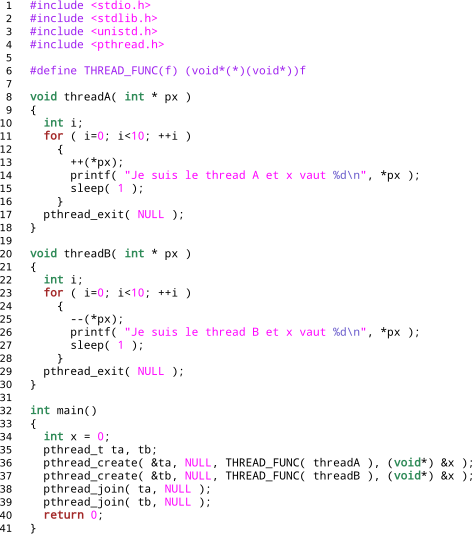
\includegraphics[width=250px]{Images/fig27.pdf} \\

\titre{Question 9} \\
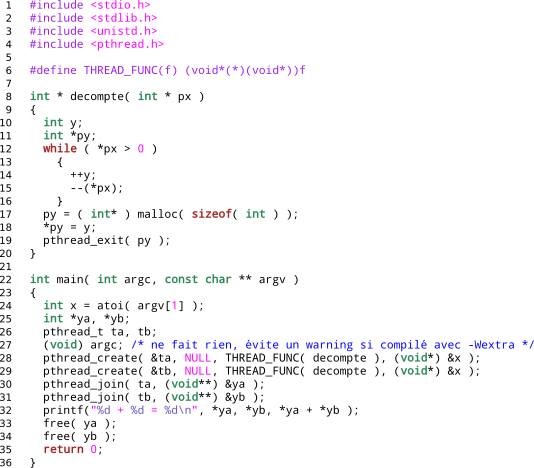
\includegraphics[width=300px]{Images/fig28.pdf} \\
